% A point p inside a metric space M, surrounded by its open
% r-neighborhood M_r(p) (dashed circle of radius r centered at p).
% Source: book/tex/topology/metric-top.tex (§ Open sets).
\documentclass[border=2mm]{standalone}
\usepackage{tikz}
\usetikzlibrary{calc}
\begin{document}
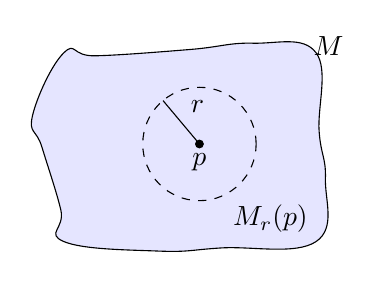
\begin{tikzpicture}[>=latex, scale=0.4]
  % Irregular "blob" silhouette of the metric space M.
  \draw[fill=blue!10, draw=black] plot[smooth cycle, tension=0.7]
    coordinates {(-4,3) (-5,1) (-4.7,0) (-4.1,-2) (-4,-3)
      (-1,-3.3) (1,-3.2) (4,-3) (4.3,-1) (4.1,0.5) (4,3)
      (2,3.3) (0,3.1) (-3,2.9)};
  \node at (4.4,3.2) {$M$};
  % The point p inside M.
  \fill (0.3,0.1) circle (4pt);
  \node[below] at (0.3,0.1) {$p$};
  % The r-neighborhood: dashed circle of radius 1.8 around p.
  \draw[dashed] (0.3,0.1) circle (1.8);
  % Label M_r(p) on the lower right of the dashed circle.
  \node[below right]
    at ($(0.3,0.1) + ({1.8*cos(-65)},{1.8*sin(-65)})$) {$M_r(p)$};
  % Radius indicator: line from p outward, with "r" label at midpoint.
  \draw (0.3,0.1) -- ($(0.3,0.1) + ({1.8*cos(130)},{1.8*sin(130)})$);
  \node[above right]
    at ($(0.3,0.1) + ({0.9*cos(130)},{0.9*sin(130)})$) {$r$};
\end{tikzpicture}
\end{document}
